%!TEX root = ../slides.tex

\section{Глиальные опухоли}

\begin{frame}
  \frametitle{Глиальные опухоли}
  %\framesubtitle{Subtitles are optional.}
  % - A title should summarize the slide in an understandable fashion
  %   for anyone how does not follow everything on the slide itself.

  \begin{itemize}
  \item \textbf{Нейроглия, или просто глия}  — совокупность вспомогательных клеток нервной ткани. 
  Составляет около 40\% объёма ЦНС.  Они составляют специфическое микроокружение для нейронов, 
  обеспечивая условия для генерации и передачи нервных импульсов, а также осуществляя часть 
  метаболических процессов самого нейрона.
  Нейроглия выполняет опорную, трофическую, секреторную, разграничительную (шванновские клетки),
  защитную функции, функцию обучения нейронов, играет важную роль в процессах памяти.
  
  \item \textbf{Астроцит}  — тип нейроглиальной 
  клетки звёздчатой формы с многочисленными отростками. Совокупность астроцитов называется астроглией.
  \item \textbf{Эпендимальные клетки} - напоминают однослойный эпителий, лежат на базальной мембране и 
  имеют кубическую или призматическую форму.
  \item\textbf{Олигодендроциты, или олигодендроглия} — вид нейроглии. Олигодендроциты есть только в центральной нервной системе, 
  которая у позвоночных включает в себя головной мозг и спинной мозг. Их главная функция — 
  предоставлять помощь и изоляцию аксонам нейронов, находящихся в центральной нервной системе позвоночных животных (аналогично шванновским клеткам в периферической нервной системе.
  
  
  % Иллюстрация четырёх типов глиальных клеток, находящихся в ЦНС: эпендимный слой (светло-розовый), астроциты (зелёный), клетки микроглии (тёмно-коричневый), олигодендроциты (голубой).
 \end{itemize}
\begin{figure}
  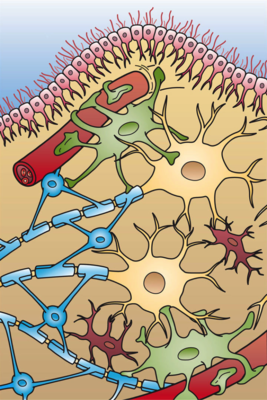
\includegraphics[scale=0.5]{glia_types.png}
\end{figure}
\end{frame}

\begin{frame}
  \frametitle{Глиальные опухоли}

  \begin{itemize}
  \item \textbf{Глиальная опухоль} является патологическим новообразованием, расположенным внутри мозга. 
    Она развивается из глии – вспомогательных клеток нервной ткани.
    
  \item \textbf{Астроцитома} — глиальная опухоль головного мозга, возникающая из астроцитов. 
  Может встречаться в любом возрасте. Опухоль бледно-розового цвета, по плотности практически не отличается от вещества мозга. 
  Отграничена от вещества мозга, однако бывают случаи, когда определить границы астроцитомы невозможно. 
  Внутри опухоли часто образуются кисты, которые растут медленно, но могут достигнуть существенно 
  больших размеров. В основном, образование кист при астроцитоме происходит у детей. 
  У взрослых астроцитома возникает чаще всего в полушариях большого мозга, у детей — в полушариях
  мозжечка в виде узлов с кистами. Наиболее характерным для астроцитомы является 
  экспансивно-инфильтративный рост.

  \item \textbf{Мультиформная глиобластома} — наиболее частая и наиболее агрессивная форма опухоли мозга,
  которая составляет до 52 \% первичных опухолей мозга и до 20 \% всех внутричерепных опухолей. 

    %Два ПЭТ изображения: верхнее показывает нормальный мозг, а нижнее — с астроцитомой.
    \begin{figure}
      \includegraphics[scale=0.5]{Astrocytoma.jpg}
    \end{figure}

  \end{itemize}
\end{frame}

\begin{frame}
  \frametitle{Глиальные опухоли}  
\begin{itemize}
  
  \item \textbf{К глиомам также относятся:}
  \begin{itemize}
    \item эпендимома — 5-8\% всех опухолей головного мозга (чаще локализуются в желудочковой системе головного мозга)
  \item астроцитома — 50 \% (располагаются обычно в белом веществе головного мозга). Различают фибриллярные (протоплазматическая, гемистоцитическая), анапластические астроцитомы, глиобластомы (гигантоклеточная, глиосаркома), пилоцитарные астроцитомы, плеоморфные ксантоастроцитомы, субэпендимарные гигантоклеточные астроцитомы
  \item олигодендроглиома — 8-10\%. К ним относятся олигодендроглиома и анапластическая олигодендроглиома
  \item смешанные глиомы (олигоастроцитома, анапластическая олигоастроцитома)
  \item опухоли сосудистого сплетения (1-2\%)
  \item невриномы (8-9\%)
  \item нейроэпителиальные опухоли неясного происхождения (астробластома, полярная спонгиобластома)
  \item глиоматоз мозга
  \item нейрональные и смешанные нейронально-глиальные опухоли — 0,5%
   \end{itemize}
  \item
  Согласно классификации ВОЗ, глиальные опухоли делятся на четыре типа. В основе этой классификации лежит 4 основных признака:
    \begin{itemize}
      \item I степень злокачественности (доброкачественная опухоль): пилоцитарная астроцитома
      \item II степень злокачественности (один признак злокачественности, как правило клеточная атипия): диффузная астроцитома 
      \item III степень злокачественности (два признака из трех, исключая некрозы): анапластическая астроцитома
      \item IV степень злокачественности (три или четыре признака, но обязательно наличие некроза): мультиформная глиобластома
    \end{itemize}
         
  \end{itemize}
  \end{frame}



\begin{frame}
  \frametitle{Симптомы и прогноз}
  \begin{itemize}
    \item Симптомы глиомы являются переменными и зависят от расположения и размера опухоли. 
    Общие жалобы включают головную боль, судороги, спутанность сознания, слабость, онемение, 
    дисбаланс или нарушения координации и изменения личности, нарушения памяти и мышления. 
    Наблюдаемая симптоматика зависит от локализации и размеров опухоли.

  \item Прогноз относительно выживаемости для данного типа опухолей ЦНС является неблагоприятным. 
  Если новообразование имеет высокий уровень злокачественности, то летальный исход наступает в 
  течение 1 года. Если новообразование не имело признаков клеточной атипии, и было 
  своевременно удалено, то не менее 80\% пациентов преодолевают рубеж пятилетней выживаемости.
  \end{itemize}
\end{frame}


\subsection{Методы обследования глиальных опухолей}

\begin{frame}
  \begin{itemize}
    \frametitle{Методы обследования глиальных опухолей}
    \item Компьютерная томография с контрастным усилением (КТ)
    \item Магнитно-резонансная томография  с контрастным усилением (МРТ)
    \item ПЭТ 
    \item Сцинтиграфия
    \item Неврологическое исследование, которое обязательно включает в себя офтальмологическую проверку остроты зрения, глазного дна и полей зрения
    \item Ангиография
  \end{itemize}
\end{frame}